\documentclass[10pt,letterpaper]{article}

% Mathematics
\usepackage{amsmath}
\usepackage{amssymb}



% Page layout
\usepackage[margin=1in]{geometry}
\usepackage{microtype}
\usepackage{comment}


\usepackage{tikz}
\usetikzlibrary{positioning}
\usepackage{pgfplots}
\usepackage{booktabs}

\pgfplotsset{compat=1.18}

% Headers and footers
\usepackage{fancyhdr}
\setlength{\headheight}{14pt}

\pagestyle{fancy}
\fancyhf{}

\fancyhead[L]{\small SICP --- Chapter 1}
\fancyhead[R]{\small Exercise 1.14}
\fancyfoot[C]{\thepage}

\renewcommand{\headrulewidth}{0.4pt}
\renewcommand{\footrulewidth}{0pt}

% Hyperlinks
\usepackage[hidelinks]{hyperref}

% Paragraph formatting
\setlength{\parindent}{0pt}
\setlength{\parskip}{6pt}

\begin{document}

\begin{center}
    {\small Structure and Interpretation of Computer Programs}\\[8pt]
    {\LARGE\bfseries Exercise 1.14}\\[6pt]
    {\large Counting Change}\\[12pt]
    {\normalsize Deepak Venkatesh}\\
    {\today}
\end{center}

\vspace{0.5em}
\hrule
\vspace{1em}

\section*{Recursion Tree}

The tree would be somewhat like this. But note the original problem has 5 kinds of coins. So ideally
there were be two nodes which would return negative amounts (excluding 50 cents and 25 cents). Figure 1
shows the simplified tree.


\begin{figure}[htbp]
\centering
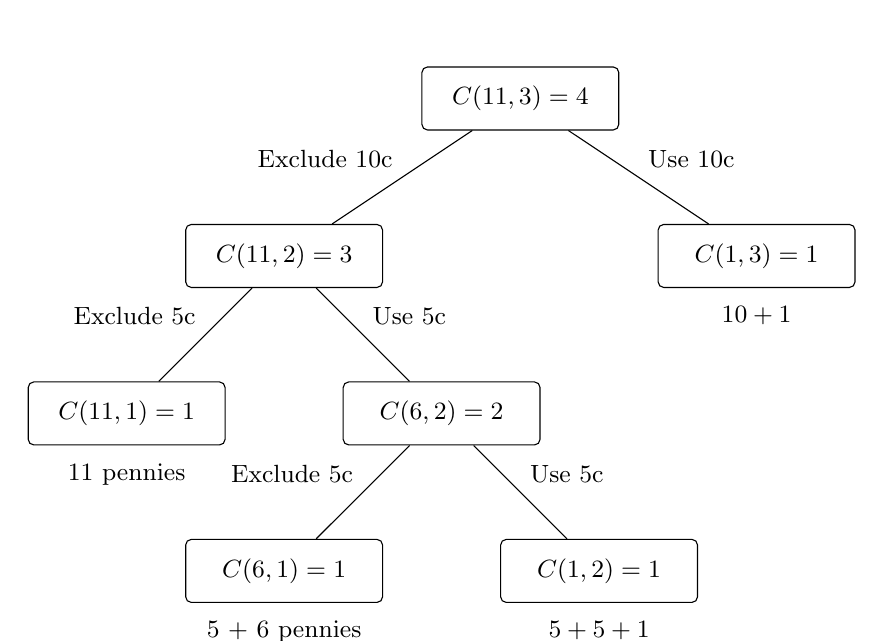
\begin{tikzpicture}[
    every node/.style={font=\small},
    process/.style={
        draw,
        rounded corners=2pt,
        minimum width=2.5cm,
        minimum height=0.8cm
    }
]

% Nodes
\node[process] (root) at (0,0)
    {$C(11,3)=4$};

\node[process] (a) at (-3,-2)
    {$C(11,2)=3$};

\node[process] (b) at (3,-2)
    {$C(1,3)=1$};

\node[process] (c) at (-5,-4)
    {$C(11,1)=1$};

\node[process] (d) at (-1,-4)
    {$C(6,2)=2$};

\node[process] (e) at (-3,-6)
    {$C(6,1)=1$};

\node[process] (f) at (1,-6)
    {$C(1,2)=1$};

% Edges
\draw (root) -- (a)
    node[midway, above left] {Exclude 10c};

\draw (root) -- (b)
    node[midway, above right] {Use 10c};

\draw (a) -- (c)
    node[midway, above left] {Exclude 5c};

\draw (a) -- (d)
    node[midway, above right] {Use 5c};

\draw (d) -- (e)
    node[midway, above left] {Exclude 5c};

\draw (d) -- (f)
    node[midway, above right] {Use 5c};

% Successful combinations
\node[below=3pt of b] {$10+1$};

\node[below=3pt of c] {11 pennies};

\node[below=3pt of e] {5 + 6 pennies};

\node[below=3pt of f] {$5+5+1$};

\end{tikzpicture}
\caption{Simplified recursion tree for counting
change for 11 cents.}
\label{fig:count-change}
\end{figure}


\section*{Algorithmic Complexity}

Let $n$ denote the amount of money to be changed
and $k$ denote the number of kinds of coins
available.

Let $d_k$ denote the denomination of the
$k$th kind of coin.

The recursive relation for counting change is

\[
    C(n,k) = C(n,k-1) + C(n-d_k,k).
\]

The terminating conditions are

\[
C(n,k) =
\begin{cases}
    1, & n=0,\\
    0, & n<0,\\
    0, & n>0 \text{ and } k=0.
\end{cases}
\]

For an amount of 11 cents, we obtain

\begin{align*}
    C(11,5)
        &= C(11,4) + C(-39,5)\\
        &= C(11,4)\\
        &= C(11,3) + C(-14,4)\\
        &= C(11,3)\\
        &= C(11,2) + C(1,3)\\
        &= 3+1\\
        &= 4.
\end{align*}

\subsection*{Space Complexity}

The space required by the recursive process is
proportional to the maximum depth of the
recursion tree.

The longest recursive path involves successive
subtractions of the smallest denomination,
which is one cent.

Since the number of denominations is fixed,

\[
    \boxed{S(n)=\Theta(n)}.
\]

\subsection*{Time Complexity}

Let $T(n,k)$ denote the number of steps required
to make change for an amount $n$ using $k$
kinds of coins.

The recurrence relation is

\[
    T(n,k) =
    T(n,k-1) + T(n-d_k,k) + \Theta(1).
\]

For a single denomination of one cent,

\[
    T(n,1)=\Theta(n).
\]

For two denominations,

\begin{align*}
    T(n,2)
        &= \Theta(n+(n-5)+(n-10)+\cdots)\\
        &= \Theta(n^2).
\end{align*}

For three denominations,

\begin{align*}
    T(n,3)
        &= \Theta(n^2+(n-10)^2+
           (n-20)^2+\cdots)\\
        &= \Theta(n^3).
\end{align*}

Generalizing for a fixed number of denominations,

\[
    T(n,k)=\Theta(n^k).
\]

Since the count-change procedure uses five
kinds of coins,

\[
    \boxed{T(n)=\Theta(n^5)}.
\]

Therefore, the orders of growth are

\[
\boxed{
\begin{aligned}
    \text{Time}  &: \Theta(n^5),\\
    \text{Space} &: \Theta(n).
\end{aligned}
}
\]

\end{document}